\documentclass[onecolumn,12pt]{article}
\usepackage[a4paper, total={7in, 9in}]{geometry}
\usepackage[utf8]{inputenc}
\usepackage[T1]{fontenc}
\usepackage{polski}
\usepackage{graphicx}
\usepackage{xcolor}
\usepackage{listings}
\usepackage{svg}


\usepackage{hyperref}
\hypersetup{
    colorlinks=false, %set true if you want colored link
    linktoc=all,     %set to all if you want both sections and subsections linked
}
\urlstyle{same}

\lstdefinestyle{yaml}{
     basicstyle=\color{blue}\footnotesize,
     rulecolor=\color{black},
     string=[s]{'}{'},
     stringstyle=\color{blue},
     comment=[l]{:},
     commentstyle=\color{black},
     morecomment=[l]{-}
 }

% Define Terraform language
\lstdefinestyle{terraform}{
  basicstyle=\footnotesize,
  keywords={resource, variable, provider, output, module, locals, terraform, backend},
  sensitive=true,
  comment=[l]{\#},
  morecomment=[s]{/*}{*/},
  morestring=[b]",
  morestring=[b]',
  keywordstyle=\color{blue}\bfseries,
  commentstyle=\color{gray}\itshape,
  stringstyle=\color{red}
}

\begin{document}

% ----------Strona tytułowa------------
\begin{titlepage}
\begin{center}
\vspace*{2.5cm}
\Huge
\textbf{Spiderpool}
            
\vspace{0.5cm}
\LARGE
RDMA network solution for the Kubernetes
            
\vspace{1.5cm}

\large
Piotr Czarnik, Bartosz Kucharz
\\Gabriela Piwar, Wojciech Szmelich
              
\vspace{0.8cm}          
\Large
AGH Wydział Informatyki\\
2024    
\end{center}
\end{titlepage}

% ----------Spis treści------------
\tableofcontents
\thispagestyle{empty}
% \newpage

% ----------Raport------------
\section{Wprowadzenie}
Kubernetes to jedno z najpopularniejszych narzędzi do zarządzania aplikacjami kontenerowymi. 
Z tego też względu nieustanie wprowadzane są nowe moduły usprawniające jego działanie. 

Jednym z nich jest Spiderpool - zaawansowane rozwiązanie zarządzania adresami IP (IPAM - IP Address Management) wykorzystujące technologię RDMA (Remote Direct Memory Access).
Rozszerza on standardowe interfejsy sieciowe kontenerów (CNI - Container Network Interface) umożliwiając tworzenie interfejsów Macvlan, Ipvlan, oraz SR-IOV.
Dzięki temu pozwala na większą dowolność w przypisywaniu adresów IP do kontenerów i w wykorzystaniu interfejsów sieciowych.
Natomiast SR-IOV umożliwia kontenerowi na bezpośredni dostęp do fizycznego interfejsu sieciowego - szybszy transfer danych między węzłami w klastrze Kubernetesa, minimalizacja opóźnienia i obciążenia procesora. 
Jest to szczególnie korzystne dla aplikacji wymagających wysokiej przepustowości i niskiego opóźnienia, 
jak aplikacje do przetwarzania dużych ilości danych, middleware, CNF (Container Network Functions) czy systemy baz danych.

\section{Opis technologii}

\subsection{Kubernetes}
Spiderpool działa na klastrach, czyli zestawie maszyn (węzłów) do uruchamiania skonteneryzowanych aplikacji. Kubernetes jest platformą open source do zarządzania takimi klastrami. Służy do zarządzania zadaniami i serwisami uruchamianymi w kontenerach, oraz umożliwia deklaratywną konfigurację i automatyzację. Najmniejsza i najprostsza jednostka w środowisku Kubernetes to pod, czyli grupa jednego lub wielu kontenerów aplikacji. 
W ''czystym'' k8s kontenery wewnątrz poda współdzielą adres IP i przestrzeń portów, zawsze są uruchamiane wspólnie w tej samej lokalizacji i współdzielą kontekst wykonawczy na tym samym węźle.

\subsection{AWS}
Spiderpool jest stworzone z myślą o działaniu na dowolnym środowisku chmurowym. Ułatwia również zarządzanie takimi rozwiązaniami jak multicloud czy chmura hybrydowa.\\
Jedną z najbardzej znanych i używanych platform chmurowych jest Amazon Web Services (AWS), która zapewnia szeroki wybór usług oraz zasobów obliczeniowych, sieciowych i przechowywania danych. Usługi Amazona są znacznie  rozbudowane i umożliwiają skonfigurowanie środowiska w taki sposób, aby było jak najbardziej dopasowane do danych potrzeb. Jedną z najważniejszych usług dostępnych w AWS jest Elastic Compute Cloud (EC2), która umożliwia elastyczne skalowanie zasobów obliczeniowych. Szerokie zastosowanie tej platformy oznacza również, że istnieje ogromna ilość informacji, dokumentacji i pomocy dostępnych dla użytkowników. Dlatego zdecydowano się wdrożyć projekt na tym środowisku.

\subsection{Terraform}
Terraform jest narzędziem do deklaratywnego konfigurowania i provisionowania infrastruktury cloud'owej z wykorzystaniem paradygmatu ,,infrastructure as a code''.
Z wykorzystaniem deklaratywnego języka HCL (HashCorp Language) pozwala na opisanie stanu końcowego instrastruktury - a doprowadzeniem jej do tego stanu zajmuje się Terraform. 

Terraform udostępnia dużą liczbę ,,provider'ów'', w tym provider dla AWS, umożliwiający konfigurowanie instancji EC2 i sieci VPC.


\subsection{Ansible}
Ansible jest silnikiem orkiestracji pozwalającym na tworzenie oprogramowania w paradygmacie ,,infrastructure as a code''.
Umożliwia automatyzację provisioningu, konfiguracji i deploymentu systemów oraz oprogramowania za pomocą Playbook-ów - zestawów tasków, które mają się wykonać na wcześniej zdefiniowanych node'ach.

Ansible udostępnia moduły dedykowane do konfiguracji AWSa i Kubernetesa.
Wartą uwagi cechą playbooków jest idempotentność operacji - taski sprawdzają, czy dane zadanie już nie zostało wykonane, a jeśli tak to go nie powtarzają - umożliwia to wielokrotne ich uruchamianie bez konieczności czyszczenia całego środowiska.

\section{Case Study - opis projektu}
Za pomocą wymienionych uprzednio technologii, dążymy do uzyskania automatycznego deploymentu środowiska Spiderpool na klastrze Kubernetesa na instancjach EC2 na chmurze AWS za pomocą Terraform'a i Ansible'a.
Do zespolenia tych dwóch narzędzi zostanie użyty skrypt bash'owy.

W ramach projektu zautomatyzowane zostaną więc:
\begin{enumerate}
    \item provisioning instrastruktury na AWS - VPC i EC2 za pomocą Terraforma,
    \item deployment K8s za pomocą Ansible,
    \item deployment Spiderpoola za pomocą kubernetesowych manifestów i Ansible,
    \item deployment przykładowej aplikacji za pomocą kubernetesowych manifestów i Ansible.
\end{enumerate}

\section{Architektura rozwiązania}
Nasz deployment składa się z następujących komponentów:
\begin{enumerate}
    \item jedna sieć publiczna (dla mastera) i dwie sieci prywatne (dla workerów).

    \item instancje EC2 skonfigurowane za pomocą terraforma:
        \begin{itemize}
            \item master z publicznym adresem IP,
            \item 4 workery z dostępem do internetu przez NAT, każdy z dwoma interfejsami sieciowymi na dwóch różnych sieciach prywatnych (do każdego interfejsu przypisana pula adresów prywatnych).
        \end{itemize}
        Wszystkie instancje są typu \texttt{t2.large} i wykorzystują system RHEL9.4.

    \item klaster kubernetesa (master i 4 workery) zdeployowany za pomocą Ansible (wykorzystujący pod spodem \texttt{kubeadm}).

    \item spiderpool skonfigurowany za pomocą kubernetesowych manifestów i Ansible - dwie różne IP pool'e dla dwóch sieci prywatnych, korzystające z adresów przypisanych do interfesjów workerów.

    \item pody z obrazem \texttt{busybox} umożliwiającym proste sprawdzenie działania sieci. 
\end{enumerate}

Na rys. \ref{fig:diagram} pokazano konfigurację klastra z dwoma workerami.

\section{Konfiguracja środowiska}

Konieczne jest systemu Linux. Należy posiadać klucz \texttt{ssh} typu \texttt{ed25519}.
Należy mieć dostęp do konsoli AWS (np. przez AWS Academy) z lokalnej maszyny - w~pliku \texttt{\~/.aws/credentials} należy umieścić dane konfiguracyjne z konsoli.

Konieczne jest zainstalowanie następujących pakietów na lokalnej maszynie:
\begin{itemize}
    \item \texttt{ansible},
    \item \texttt{terraform},
    \item \texttt{helm},
    \item \texttt{kubectl}.
\end{itemize}
Dodatkowo po zainstalowaniu \texttt{ansible}, należy doinstalować moduły do kubernetesa:
\begin{verbatim}
    ansible-galaxy collection install kubernetes.core
    pip install "Jinja2<3.1"
    pip install kubernetes
\end{verbatim}

\section{Instalacja}

Należy sklonować repozytorium i uruchomić skrypt \texttt{provision\_and\_deploy.sh}, który przeprowadzi proces provisioningu instancji, deployment kubernetesa, spiderpoola i przykładowej aplikacji.

\begin{verbatim}
    git clone https://github.com/gpiwar/suu_spiderpool_project.git
    cd suu_spiderpool_project
    ./provision_and_deploy.sh
\end{verbatim}

Skrypt ten uruchamia po kolei następujące komendy - w razie przerwania lub napotkania błędu można wznowić deployment wykorzystując następujące komendy:
\begin{verbatim}
    cd terraform
    terraform init
    terraform apply --auto-approve
    cd -

    ansible-playbook -i ansible/inventory/hosts.cfg ansible/pre-deploy.yml
    ansible-playbook -i ansible/inventory/hosts.cfg ansible/deploy-k8s.yml
    ansible-playbook -i ansible/inventory/hosts.cfg ansible/deploy-spiderpool.yml
    ansible-playbook -i ansible/inventory/hosts.cfg ansible/deploy-apps.yml
\end{verbatim}

\begin{figure}[!htpb]
    \centering
    \includesvg[width=\linewidth]{imgs/spiderpool.svg}
    \caption{Schemat przedstawiający oczekiwaną konfigurację.}
    \label{fig:diagram}
\end{figure}

\section{Opis provisioningu i deploymentu}

\subsection{Terraform}
Terraform provisionuje instancje EC2 i tworzy sieci (w tym tablice routingu, NAT i Internet Gateway'e, security groupy).
Na rysunku \ref{fig:diagram} przedstawiono konfigurację sieci i instancji EC2.

\subsubsection{Sieć}
Tworzone są 3 sieci: 
\begin{itemize}
    \item jedna publiczna \texttt{172.31.0.0/20},
    \item dwie prywatne \texttt{172.31.64.0/20} i \texttt{172.31.96.0/20}.
\end{itemize}

Tworzone są interfejsy sieciowe, dla każdego z workerów po dwa (eth0 i eth1, z dwóch sieci prywatnych).
Każdy interfejs ma pulę adresów IP.

\subsubsection{Security groups}
Master korzysta z security group'y z otwartym portem ingress dla ssh.
Dla sieci prywatnych dla workerów jest stworzona osobna security group'a z otwartymi wszystkimi portami (ingress i egress) - jedynie w celu ułatwienia developmentu PoC.

\subsubsection{Instancje}
\paragraph{master} posiada publiczny adres IP i zarządza całym klastrem kubernetes.
\paragraph{workery} posiadają dwa interfejsy sieciowe - eth0 i eth1 podłączone do dwóch różnych sieci prywatnych - każdy z interfejsów ma przypisaną pulę adresów IP (rys. \ref{fig:worker1-ips}).

\begin{figure}[!htpb]
    \centering
    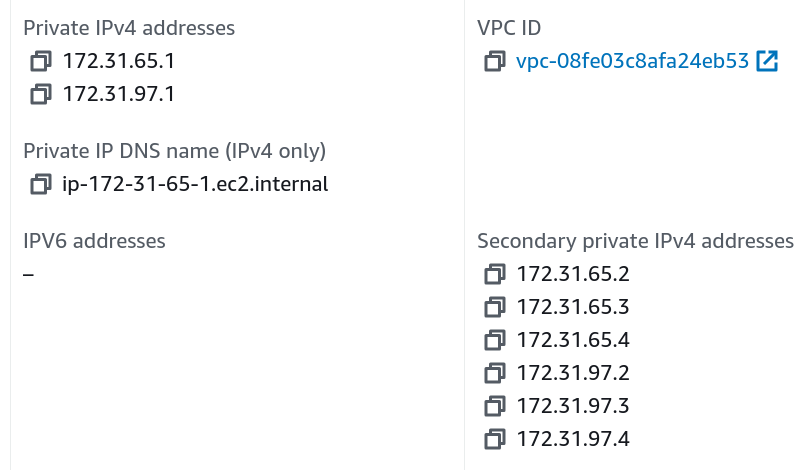
\includegraphics[width=0.6\linewidth]{imgs/aws-console-ifs.png}
    \caption{Adresy IP przypisane do workera 1.}
    \label{fig:worker1-ips}
\end{figure}

\subsection{Playbooki Ansible}
\subsubsection{pre-deploy.yml}
Dokonujemy konfiguracji połączenia z master i workerami.
Dodajemy klucz ssh, ustawiamy hostname'y, dodajemy adresy IP do /etc/hosts.
W wyniku tego kroku uzyskujemy dostęp do jeszcze nie skonfigurowanego klastra - punktem wejścia jest master z publicznym IP. Do zalogowania się należy użyć użytkownika \texttt{ec2-user}.

\subsubsection{deploy-k8s.yml}
Przygotowujemy node'y pod kubernetesa (wyłączenie SELinux i swap'u, włączenie modułów kernela).
Instalujemy CRI-O i kubelet, następnie uruchamiamy je.

Następnie na masterze pobieramy obrazy dla kubernetesa i inicjalizujemy mastera za pomocą \texttt{kubeadm} z endpointem na publicznym IP mastera - umożliwi to dostęp do klastra za pomocą komend kubectl z poziomu lokalnej maszyny użytkownika.
Po inicjalizacji mastera, dodajemy workery do klastra.

W wyniku tego kroku otrzymujemy działajacy klaster kubernetesa, co można sprawdzić wykonując komendy:
\begin{verbatim}
    $ export KUBECONFIG="./kubeconfig"
    $ kubectl get nodes
    NAME      STATUS   ROLES           AGE   VERSION
    master    Ready    control-plane   3m    v1.30.2
    worker1   Ready    <none>          1m    v1.30.2
    worker2   Ready    <none>          1m    v1.30.2
    worker3   Ready    <none>          1m    v1.30.2
    worker4   Ready    <none>          1m    v1.30.2
\end{verbatim}

\subsubsection{deploy-spiderpool.yml}
Za pomocą helm-a instalujemy spiderpool-a.
Dodajemy dwie konfiguracje ipvlan dla spiderpool-multusa - dla interfejsów eth0 i eth1.
Następnie dodajemy pule adresów IP.
Powyższe jest równoznaczne ręcznemu zaplikowaniu manifestów:
\begin{verbatim}
    kubectl apply -f manifests/SpiderMultusConfig.yaml
    kubectl apply -f manifests/SpiderIPPool.yaml
\end{verbatim}

W wyniku tego kroku uzyskujemy działającego spiderpoola z pulami adresów IP:
\begin{verbatim}
    $ kubectl get spidermultusconfigs.spiderpool.spidernet.io -n kube-system
    NAME          AGE
    ipvlan-eth0   22m
    ipvlan-eth1   22m
    $ kubectl get spiderippools
    NAME          VERSION   SUBNET           ALLOCATED-IP-COUNT   TOTAL-IP-COUNT
    172-31-64-0   4         172.31.64.0/20   0                    16
    172-31-96-0   4         172.31.96.0/20   0                    16
\end{verbatim}

\subsubsection{deploy-apps.yml}
Deployujemy prostą aplikację z obrazem busybox, pozwalającą na sprawdzenie przydziału adresów IP do interfejsów podów.
\begin{verbatim}
    kubectl apply -f manifests/Deployment-busybox.yaml
\end{verbatim}
W wyniku tego uzyskujemy 4 pody, każdy z nich ma dwa interfejsy sieciowe: eth0 i net1.
\begin{verbatim}
    $ kubectl get pods -owide
    NAME                       READY   STATUS    AGE   IP            NODE
    busybox-5dc5cb4bf6-6kv5d   1/1     Running   24m   172.31.65.3   worker1
    busybox-5dc5cb4bf6-9hxxb   1/1     Running   24m   172.31.66.2   worker2
    busybox-5dc5cb4bf6-9jsts   1/1     Running   24m   172.31.68.1   worker4
    busybox-5dc5cb4bf6-9ml79   1/1     Running   24m   172.31.67.4   worker3
    $ kubectl exec -it busybox-5dc5cb4bf6-6kv5d -- ip -4 addr show scope global
    2: eth0@eth0: <BROADCAST,MULTICAST,UP,LOWER_UP> mtu 9001 qdisc noqueue 
        inet 172.31.65.3/20 brd 172.31.79.255 scope global eth0
           valid_lft forever preferred_lft forever
    4: net1@veth0: <BROADCAST,MULTICAST,UP,LOWER_UP> mtu 9001 qdisc noqueue 
        inet 172.31.97.3/20 brd 172.31.111.255 scope global net1
           valid_lft forever preferred_lft forever
\end{verbatim}

\subsection{Dodatkowa konfiguracja}

Nasz deployment charakteryzuje się dosyć dużą swobodą w konfiguracji kubernetesa i spiderpoola.
Użytkownik może:
\begin{itemize}
    \item dodać lub usunąć workery do klastra - plik \texttt{terraform/variables.tf}, sekcja \texttt{locals/workers}. Przykładowy 5. worker:
    \begin{verbatim}
    worker5 = {
      ami           = data.aws_ami.this.id
      instance_type = "t2.large"
      interfaces = [
        aws_network_interface.this["worker5_eth0"].id,
        aws_network_interface.this["worker5_eth1"].id
      ]
    }
    \end{verbatim}

    \item dodać interfejsy do workerów i przypisać im adresy z sieci prywatnych - \texttt{terraform/variables.tf}, sekcja \texttt{locals/interfaces}. Przykładowy interfejs dla worker5:
    \begin{verbatim}
    worker5_eth1 = {
      subnet_id = aws_subnet.private[1].id
      ip_list   = [for i in range(1, 5) : "172.31.101.${i}"]
    }
    \end{verbatim}

    \item zmodyfikować sieci prywatne - \texttt{terraform/variables.tf}, sekcja \texttt{private\_subnet\_cidrs}.
    \begin{verbatim}
    variable "private_subnet_cidrs" {
      type        = list(string)
      description = "Private Subnet CIDRs"
      default     = ["172.31.64.0/20", "172.31.96.0/20"]
    }
    \end{verbatim}

    \item dodać pule adresów przypisanych do workera do spiderpoola - \texttt{manifests/SpiderIPPool.yaml}:
    \begin{verbatim}
    kind: SpiderIPPool
    metadata:
      name: 172-31-96-0
    spec:
      subnet: 172.31.96.0/20
      ips:
        ...
        - 172.31.101.1-172.31.101.4
      gateway: 172.31.96.1
      default: true
      multusName: ["kube-system/ipvlan-eth1"]
    \end{verbatim}
\end{itemize}




\section{Podsumowanie}
Nasz projekt automatyzuje provisioning infrastruktury AWS i deployment klastra kubernetes z pluginem spiderpool.
Wykorzystuje do tego paradygmat ,,infrastructure as a code'':
Z wykorzystaniem Terraforma provisionuje instancje AWS EC2, tworzy i konfiguruje sieci na AWS VPC.
Następnie za pomocą Ansible'a deployuje klaster kubernetesa na stworzonych wcześniej instancjach EC2.
Na tak skonfigurowanym klastrze deployowany jest spiderpool z dwoma pulami adresów IP.
Na sam koniec uruchamiana jest przykładowa aplikacja z czterema podami, z których każdy ma dwa interfejsy sieciowe z adresami IP z różnych sieci prywatnych.

W ramach testów wielokrotnie sprawdzono poprawność alokacji adresów IP w utworzonych podach.

%\bibliography{}

\end{document}